\section{Durchführung und Auswertung}

\subsection{LABVIEW-Messprogramm}

Wir haben zur Messung das bereits vorhandene Messprogramm verwendet. Allerdings zeigte sich im Laufe der Messungen, dass die Qualität gesteigert werden kann, wenn zwischen den einzelnen Messungen die Hochspannung auf $0V$ heruntergefahren wird. Durch das Methan können dann verbleibende Ionen anscheinend besser herausgespült werden. Daher haben wir das Programm um diese "`Reinigungsphase"' erweitert.

\subsection{Einstellen der Messelektronik}

TODO!

\subsection{Zählrohrcharakteristik}

Wir haben damit begonnen, die Zählrohrcharakteristik aufzunehmen. Dazu haben wir eine \atom{238}{}{U} Probe verwendet, die eine gute Zählrate zeigt.

\begin{figure}[H]
 \centering 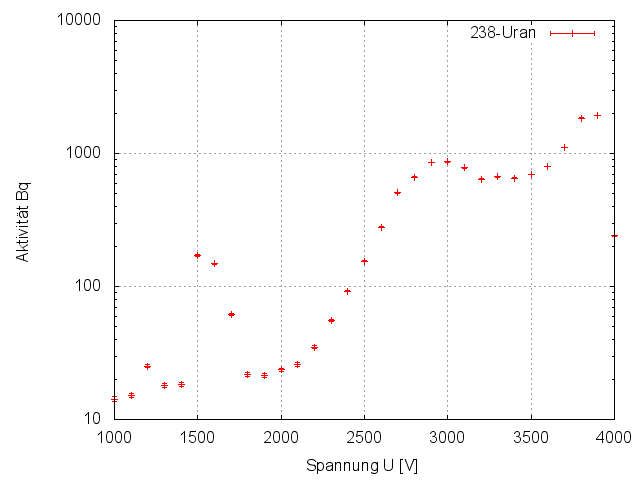
\includegraphics[width=0.9\linewidth]{Messwerte/plots/U238.png}
 \caption{Zählrohrcharakteristik, gemessen mit \atom{238}{}{U}}
\end{figure}
Als Parameter haben wir dabei gesetzt: $U = 1kV \cdots 4kV$, $\Delta U = 100 V$, $t = 50s$ sowie $t_{Pause} = 10s$

Der Graph zeigt den erwarteten Verlauf, abgesehen von einigen Ausreisern am Anfang des $\alpha$-Plateaus. \atom{238}{}{U} zerfällt durch $\alpha$-Zerfall in \atom{234}{}{Th} (Thorium). Dieses zerfällt mit einer Halbwertszeit $T_{1/2} = 24.10d$ durch einen $\beta^-$-Zerfall in \atom{234}{}{Pa} (Proactinium), welches ebenfalls durch $\beta^-$-Zerfall in \atom{234}{}{U} zerfällt. Deshalb sehen wir in der Zählrohrcharakteristik sowohl ein Plateaubereich, in dem haupsächlich $\alpha$-Strahlung detektiert wird bei ca. $U = 1100V$ bis $U = 2100V$ als auch einen Plateaubereich in dem $\alpha$- und $\beta$-Strahlung detektiert werden zwischen $3000V$ und $3700V$.

Auf das Abziehen des Untergrundes haben wir verzichtet, einerseits da der Untergrund eine Aktivität von ca. $0.001Bq$ bis maximal $1.0Bq$ zeigte, also deutlich weniger als die eigentliche Intensität. Andererseits sind die Ergebnisse der Untergrundmessung eh fraglich, wie später erleutert wird.

\subsection{Bestimmung der Halbwertszeit von \atom{147}{}{Sm} ($\alpha$-Zerfall)}

Wir haben für den im voherigen Versuchsabschnitt ermittelten $\alpha$-Plateaubereich eine grobe Messung mit einer \atom{147}{}{Sm}-Probe vorgenommen. Die Parameter dafür waren: $U= 1000V \cdots 3300V$, in $\Delta U = 100 V$ Schritten mit $t=200s$ und $t_{Pause} = 10s$.

\begin{figure}[H]
 \centering 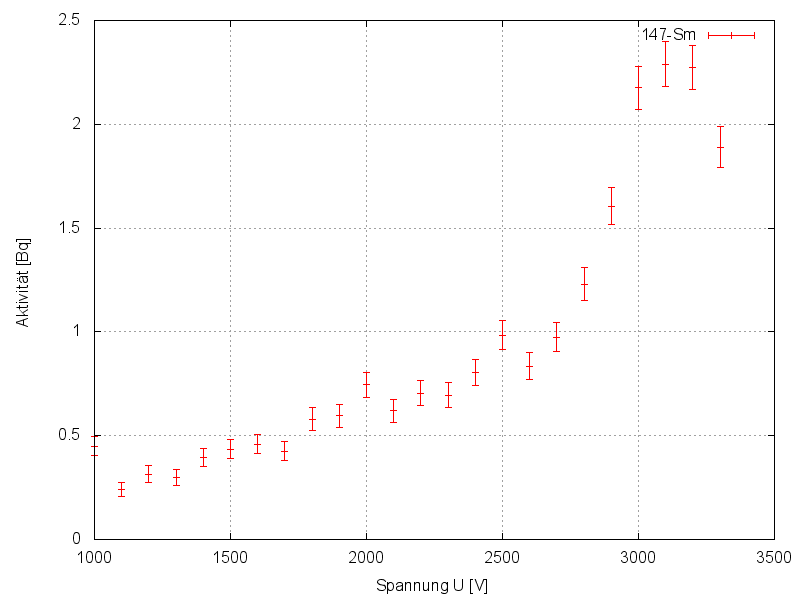
\includegraphics[width=0.9\linewidth]{Messwerte/plots/Sm147_plateau.png}
 \caption{Plateaubereich, gemessen mit \atom{147}{}{Sm}}
\end{figure}

TODO: Fehlerrechnung erläutern?

Die Mitte des Plateaus liegt also bei etwa $U_{\alpha} = 2000 V$. Bei dieser Spannung betrug die Zählrate $n = 0.745$, die durchschnittliche Zählrate auf dem Plateau lag aber eher bei $\overline{n} = 0.6$, so dass wir zur Abschätzung der benötigten Messzeit diesen Wert verwendet haben. Über die Gleichung \ref{zeitfuerkleinenfehler} ermitteln wir, dass unsere Messung mindestens $t_{0.02} = 4168 s$ dauern sollte. Wir führen daher eine Messung mit $t = 4200s$ und $ U = 2000 V$ durch. Dabei erhalten wir eine Zählrate von $n = 0.39 Bq$. Diese Zählrate ist wesentlich niedriger als der von uns erwartete Wert und kann auch nur sehr schwer durch statistische Schwankungen begründet werden. Auch zwei kürzere ($t = 60s$) Kontrollmessungen ergeben wieder deutlich höhere Zählraten ($n_1 = 0.650$ und $n_2 = 0.633$). Als Hauptfehlerquellen stuffen wir die Gaszufuhr und die Hochspannung ein. Bei genauerem Betrachten der Gasableitung ist uns dann aufgefallen, dass sich im Schlauch das Gas in Form von Blasen fortbewegt. Also haben wir den Schlauch entfernt und festgestellt, dass er mit Öl (und \atom{40}{}{K}-Krümmeln) gefüllt war, welches vermutlich aus dem Bläschenzähler stammt, durch zu hohe Gaszufuhr mitgerissen wurde und sich im Schlauch wieder ablagerte. Nach Reinigung des Schlauches war der Abfluss des Gases nun wieder deutlich konstanter. Wir führten also erneut eine Messung mit $t=4200s$ durch und erhielten diesmal eine realistischere Zählrate von $n = 0,611 Bq$ (also $N = 2565$). 

Für die Berechnung der Halbwertszeit $t_{1/2}$ haben wir weiterhin den Innendurchmesser der Aluschale gemessen und $d = (290.125 \pm 0.125) mm$ erhalten.

Todo: T1/2 berechnen!

\subsection{Halbwertszeit von \atom{40}{}{K} ($\beta$-Zerfall) - Teil 1}

Für die Messung der Halbwertszeit von \atom{40}{}{K} haben wir das $\beta$-Plateau im Bereich von $U = 2900V \cdots 4000V$ in $\Delta U = 100 V$-Schritten je $t=100s$ lang vermessen. Dazu verwendeten wir $m=1.2158g$ Kalium.

\begin{figure}[H]
 \centering 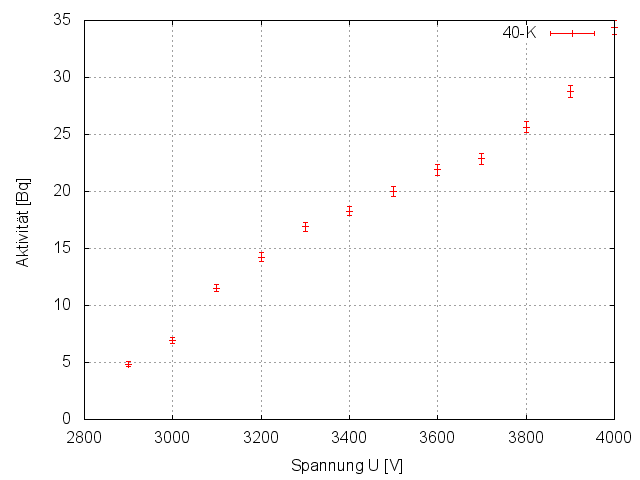
\includegraphics[width = 0.99\linewidth]{Messwerte/plots/K40_plateau.png}
 \caption{\atom{40}{}{K}-Plateau}
 \label{k40plateau}
\end{figure}

Die Mitte des Plateaus liegt also wie in Abb \ref{k40plateau} sichtbar bei etwa $U = 3600V$, wobei die Zählrate dort etwa $n = 22 Bq$ beträgt. Daraus ergibt sich eine minimale Messdauer von $t_{0.02} = 113.6 s$. Wir haben also die bereits für die Plateaumessung verwendete Probe mit $m = 1.2158g$ nochmals für $t = 120s$ vermessen. Dabei erhielten wir in zwei Messungen Zählraten von $n_1 = 9620.017 Bq$ bzw. $n_2 = 31 202.083 Bq$. Diese unrealistischen Werte könnten z.B. durch Übergang in den Gasentladungsmodus, Verbleiben von Ionen im Zählrohr, eine zu niedrig eingestellte Diskriminatorschwelle oder Defekte der Messelektronik/Software entstehen. Bie einer dritten Messung, nach einem Reset der Spannung, gelang uns wieder eine vernünftige Messung mit einer Zählrate $n = 5.708 Bq$. Da diese jedoch der Plateaumessung deutlich widersprach, haben wir diese ebenfalls wiederholt. Dabei haben wir wieder $U = 2900V \cdots 4000V$ in $\Delta U = 100 V$-Schritten je $t=100s$ als Parameter verwendet. 


\begin{figure}[H]
 \centering 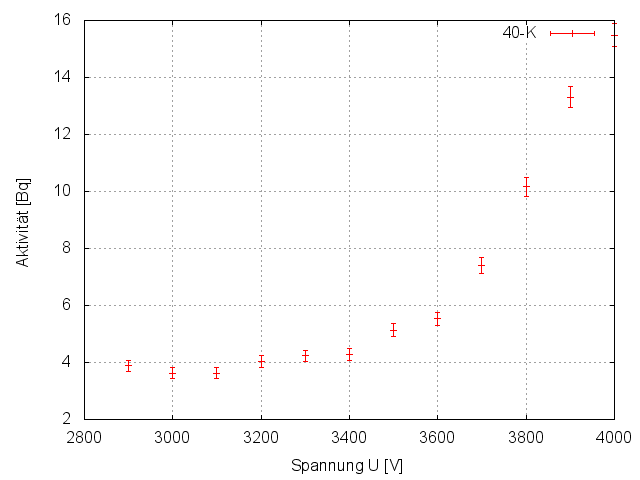
\includegraphics[width = 0.99\linewidth]{Messwerte/plots/K40_plateau2.png}
 \caption{\atom{40}{}{K}-Plateau}
\end{figure}

\subsection{Untergrundmessung}
Über das Wochenende haben wir eine ausführliche Untergrundmessung vorgenommen. Dazu haben wir das angepasste Messprogramm verwendet, und Messungen von $U = 0V \cdots 4000V$ mit $\Delta U = 50V$. Die Dauer der Einzelmessungen stellten wir auf $t=3000s$ mit einer Pause von $t_{Pause} = 60 s$ sowie einer gleichlangen Zeit für das Einstellen der Spannung.

\begin{figure}[H]
 \centering 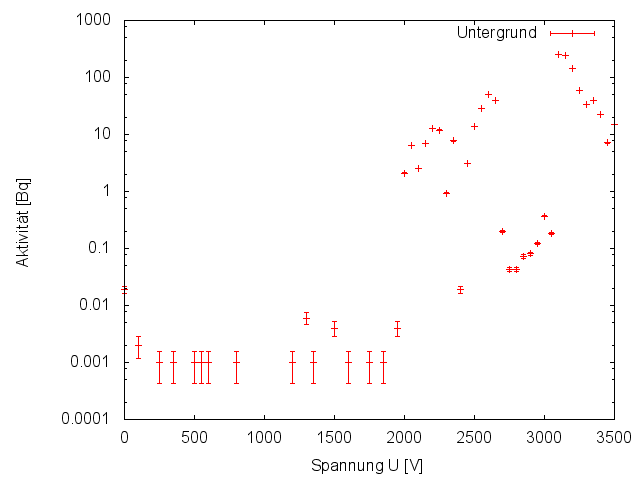
\includegraphics[width = 0.99\linewidth]{Messwerte/plots/untergrund_we.png}
 \caption{Untergrundmessung}
\end{figure}

Am Montag mussten wir leider feststellen gleich mehrere Probleme feststellen. Erstens hatten wir uns verrechnet, die Messung wäre erst am Montag abend fertig gewesen. Zweitens war die Gaszufuhr versiegt, es waren trotz geöffnetem Hahn keine Blasen mehr zu sehen im Durchflusszähler und drittens waren die Zählraten häufig und ab ca 3400V dann konsequent zu hoch. Wir haben daher beschlossen, Zählraten mit $ n > 1 Bq$ zu verwerfen. Diese Grenze haben wir einerseits aus dem Vergleich mit den Messungen mit Präparat und andererseits aus den durchschnittlichen Untergrundmesswerten ermittelt.

\begin{figure}[H]
 \centering 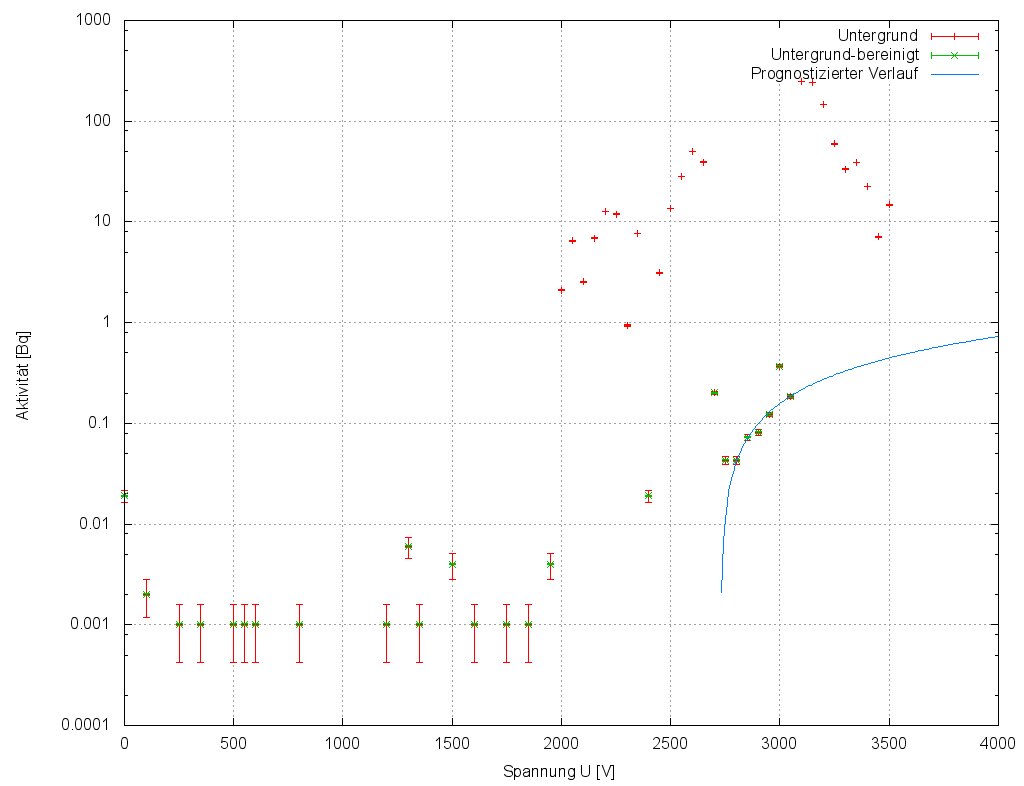
\includegraphics[width = 0.99\linewidth]{Messwerte/plots/untergrund_we_bereinigt.png}
 \caption{Untergrundmessung}
\end{figure}

